\documentclass[../thesis.tex]{subfiles}

\begin{document}
\vspace{-1\baselineskip}

\section{Event selection}
Events for the analysis first are preselected following a list of criteria to optimize for event quality and background rejection. The following criteria are applied sequentially from top to bottom along with cleaning and veto cuts

\begin{enumerate}
\item \textbf{Good Run List (\acs{GRL})}: data events must be part of a predefined list of suitable runs and luminosity blocks \citep{sample:data}.
%\item \textbf{Calorimeter cleaning}: events containing signal hits indicating an error in the calorimeter are removed.
\item \textbf{Primary vertex}: events must have at least one reconstructed vertex matched to 2 or more associated tracks with $\pT>500$ MeV.
\item \textbf{Trigger}: events must be selected by at least one trigger in \autoref{tab:ana:trigger}.
%\item \textbf{Jet cleaning}: events must pass the LooseBad WP for jet cleaning using jets passing preselection criteria in \autoref{sec:objdef}. This is done to remove events with significant number of calorimeter hits from non-prompt sources (e.g. instrumental effects, cosmic ray background, non-collision particles)
%\item \textbf{Bad muon veto}: events are removed if they contain at least one muon before overlap removal with insufficient \pT resolution.
\item \textbf{Kinematic selection}: events must have exactly two \textit{Tight} leptons with the same electric charge, or at lease three \textit{Tight} leptons of any charge. The leading lepton must have $\pT>28$ GeV, and all leptons must satisfy $\pT>15$ GeV.
\end{enumerate}

Events are separated into two channels based on the number of leptons: same-sign di-lepton (\acs{SS2L}) for events with exactly two leptons of the same charge, or multilepton (\acs{ML}) for events with three or more leptons. The channels are further separated into regions defined in \autoref{sec:ana} to prepare for analysis.

Additional selections are applied based on the lepton flavors present. In the SS2L channel, if both leptons are electrons, the invariant mass $m_{ll}$ must satisfy $m_{ll}<81$ GeV and $m_{ll}>101$ GeV to suppress background involving $Z$-bosons. In the \acs{ML} channel, the same criteria must be satisfied for every opposite-sign same-flavor pair of leptons in an event.

\subsection{Object definition}
\label{sec:objdef}
\autoref{tab:obj_sel} shows the selections used in this analysis. Each selection comes with associated calibration scale factors (\acs{SF}s) to account for discrepancies between data and \acs{MC} simulation, and are applied multiplicatively to \acs{MC} event weights.

\begin{table}[!htp]
\centering
\caption{\label{tab:obj_sel}Summary of object selection criteria used in this analysis.}%
\begin{tabular}{l|cccc}
\toprule\toprule
Selection			& Electrons	& Muons		& Jets	\\
\midrule
\midrule
\multirow{ 2}{*}{\pT [GeV]}
	& $>15$ 					& $>15$ 	& $>20$ \\
	& $\pT (l_0)>28$ & & &  \\
\midrule
\multirow{ 2}{*}{$|\eta|$}
	& $1.52\leq|\eta|<2.47$ 	& $<2.5$ 	& $<2.5$ \\
	& $<1.37$ & & &  \\
\midrule
\multirow{ 2}{*}{Identification}
	& \textit{TightLH} 			& \textit{Medium} & NNJvt \textit{FixedEffPt} \\
	& pass \acs{ECIDS} ($ee$/$e\mu$) & 	& ($\pT<60$, $|\eta|<2.4$) \\
\midrule
Isolation
	& \textit{Tight\_VarRad} 	& \textit{PflowTight\_VarRad}	& \\
\midrule
Track-vertex assoc.\vphantom{$\frac{1}{p}$} & & & \\
\hspace{3mm} $|d_0^{\text{BL}}(\sigma)|$ 
	& $<5$ 		& $<3$ 		& \\
\hspace{3mm} $|\Delta z_0^{\mathrm{BL}}\sin\theta|$ [mm]
	& $<0.5$ 	& $<0.5$ 	& \\
\bottomrule\bottomrule
\end{tabular}
\end{table}

\subsection{Event categorization}
Simulated events are categorized using truth information of leptons ($e$/$\mu$) and their originating \acs{MC} particle (mother-particle). Each lepton can be classified as either prompt or non-prompt, with non-prompt leptons further categorized for background estimation purposes. If an event contains only prompt leptons, the event is classified as its corresponding process. If the event contains one non-prompt lepton, the event is classified as the corresponding type of the non-prompt lepton. If the event contains more than one non-prompt lepton, the event is classified as other.

\begin{itemize}
\item \textbf{Prompt}: if the lepton originates from $W$/$Z$/$H$ boson decays, or from a mother-particle created by a final state photon.
\item \textbf{Non-prompt}:
	\begin{itemize}
	\item \textbf{Charge-flip ($e$ only)}: if the reconstructed charge of the lepton differs from that of the first mother-particle.
	\item \textbf{Material conversion ($e$ only)}: if the lepton originated from a photon conversion and the mother-particle is an isolated prompt photon, non-isolated final state photon, or heavy boson.
	\item \textbf{$\gamma^*$-conversion ($e$ only)}: if the lepton originated from a photon conversion and the mother-particle is a background electron.
	\item \textbf{Heavy flavor decay}: if the lepton originated from a $b$- or $c$-hadron.
	\item \textbf{Fake}: if the lepton originated from a light- or $s$-hadron, or if the truth type of the lepton is hadron.
	\item \textbf{Other}: any lepton that does not belong to one of the above categories.
	\end{itemize}
\end{itemize}

\section{Analysis regions}
\label{sec:ana}
Events are selected and categorized into analysis regions belonging to one of two types: control regions (\acs{CR}s) enriched in background events, and signal regions (\acs{SR}s) enriched in signal events. This allows for the examination and control of backgrounds and systematic uncertainties, as well as study of signal sensitivities. The signal is then extracted from the \acs{SR}s with a profile \acs{LH} fit using all regions. The full selection criteria for each region are summarized in \autoref{tab:ana_regions}.

\begin{table}[!htbp]
\centering
\caption{\label{tab:ana_regions}Definitions of signal, control and validation regions (\acs{VR}) used in this analysis. $N_\mathrm{jets}$ and $N_b$ refers to the number of jets and number of $b$-tagged jets respectively. $\ell_1$ refers to the leading lepton, $\ell_2$ refers to the subleading lepton and so on. \HT refers to the \pT scalar sum of all leptons and jets in the event. \acs{mll} refers to the dilepton invariant mass, which must not coincide with the $Z$-boson mass range of 81-101 GeV for \acs{SS2L}+3L events.}%
\resizebox{\textwidth}{!}{%
\begin{tabular}{l|lllll}
\toprule\toprule
Region & Channel & $N_\mathrm{jets}$ & $N_b$ & Other selections & Fitted variable \\
\midrule
\midrule
\multirow{2}{*}{CR Low $m_{\gamma^{*}}$}	& \multirow{2}{*}{SS $e\ell$} 	& \multirow{2}{*}{$[4,6)$}	& \multirow{2}{*}{$\geq 1$}	&
	$\ell_1/\ell_2$ is from virtual photon decay 	& \multirow{2}{*}{event yield} \\
	& & & & $\ell_1+\ell_2$ not from material conversion & \\[6pt]
CR Mat. Conv. 			& SS $e\ell$ 	& $[4,6)$	& $\geq 1$	&
	$\ell_1/\ell_2$ is from material conversion 	& event yield \\[6pt]
\multirow{4}{*}{CR HF $\mu$} 			& \multirow{4}{*}{$\ell\mu\mu$} 	& \multirow{4}{*}{$\geq 1$}	& \multirow{4}{*}{$1$}		&
	$\ell_1+\ell_2$ not conversion candidates & \multirow{4}{*}{$\pT(\ell_3)$} \\
	& & & & $100 < \HT < 300$ GeV & \\
	& & & & $\ETmiss > 35$ GeV & \\
	& & & & total charge $= \pm 1$ & \\[6pt]
\multirow{4}{*}{CR HF $e$} 				& \multirow{4}{*}{$ee\ell$}		& \multirow{4}{*}{$\geq 1$}	& \multirow{4}{*}{$1$}		&
	$\ell_1+\ell_2$ not conversion candidates & \multirow{4}{*}{$\pT(\ell_3)$} \\
	& & & & $100 < \HT < 275$ GeV & \\
	& & & & $\ETmiss > 35$ GeV & \\
	& & & & total charge $= \pm 1$ & \\[6pt]
\multirow{4}{*}{CR \ttWplus}	 		& \multirow{4}{*}{SS $\ell\mu$}	& \multirow{4}{*}{$\geq 4$}	& \multirow{4}{*}{$\geq 2$}	&
	$|\eta(e)|<1.5$ & \multirow{4}{*}{$N_\mathrm{jets}$} \\
	& & & & for $N_b=2$: $\HT < 500$ GeV or $N_\mathrm{jets}<6$ & \\
	& & & & for $N_b\geq 3$: $\HT < 500$ GeV & \\
	& & & & total charge $> 0$ & \\[6pt]
\multirow{4}{*}{CR \ttWminus}			& \multirow{4}{*}{SS $\ell\mu$}	& \multirow{4}{*}{$\geq 4$}	& \multirow{4}{*}{$\geq 2$}	& 
	$|\eta(e)|<1.5$ & \multirow{4}{*}{$N_\mathrm{jets}$} \\
	& & & & for $N_b=2$: $\HT < 500$ GeV or $N_\mathrm{jets}<6$ & \\
	& & & & for $N_b\geq 3$: $\HT < 500$ GeV & \\
	& & & & total charge $< 0$ & \\[6pt]
\multirow{3}{*}{CR 1b(+)} 				& \multirow{3}{*}{SS2L+3L}		& \multirow{3}{*}{$\geq 4$}	& \multirow{3}{*}{$1$}		& 
	$\ell_1+\ell_2$ not from material conversion & \multirow{3}{*}{$N_\mathrm{jets}$} \\
	& & & & $\HT > 500$ GeV & \\
	& & & & total charge $> 0$ & \\[6pt]
\multirow{3}{*}{CR 1b(-)} 				& \multirow{3}{*}{SS2L+3L} 		& \multirow{3}{*}{$\geq 4$}	& \multirow{3}{*}{$1$}		& 
	$\ell_1+\ell_2$ not from material conversion & \multirow{3}{*}{$N_\mathrm{jets}$} \\
	& & & & $\HT > 500$ GeV & \\
	& & & & total charge $< 0$ & \\
\midrule
VR \ttZ 		& 3L $\ell^{\pm}\ell^{\mp}$	& $\geq 4$ 	& $\geq 2$ 	
	& $m_{\ell\ell} \in [81,101]$ GeV	& $N_\mathrm{jets}$, $m_{\ell\ell}$ \\[6pt]
VR \ttW+1b 	& SS2L+3L 	& 			& 			
	& CR $t\bar{t}W^{\pm}$ $||$ CR 1b($\pm$) 			& $N_\mathrm{jets}$ \\[6pt]
VR \ttW+1b+SR 	& SS2L+3L 	& 			& 			
	& CR $t\bar{t}W^{\pm}$ $||$ CR 1b($\pm$) $||$ SR 	& $N_\mathrm{jets}$ \\[6pt]
\midrule
\midrule
\multirow{2}{*}{SR} 					& \multirow{2}{*}{SS2L+3L} 		& \multirow{2}{*}{$\geq 6$}	& \multirow{2}{*}{$\geq 2$}	& 
	$\HT > 500$ GeV & \multirow{2}{*}{\HT} \\
	& & & & $m_{\ell\ell} \notin [81,101]$ GeV & \\
\bottomrule\bottomrule
\end{tabular}}
\end{table}

\subsection{Signal regions}
All events selected for the \acs{SR} must satisfy the following criteria:
\begin{itemize}
\item Contains 6 or more jets, with at least 2 jets $b$-tagged at the 85\% \acs{OP}.
\item Scalar sum of the transverse momenta of all leptons and jets $\HT > 500$ GeV.
\item Dilepton invariant mass \acs{mll} does not coincide with the $Z$-boson mass range of $81-101$ GeV
\end{itemize}
The \acs{SR} is further divided into sub-regions by the number of $b$-jets and leptons as shown in \autoref{tab:ana:SR} to further study signal behavior and improve sensitivity.

\begin{table}[!ht]
\centering
\caption{\label{tab:ana:SR}Definitions of \acs{SR} sub-regions. Events are sorted into different sub-regions based on the number of $b$-tagged jets and leptons present.}%
\begin{tabular}{p{2cm}|p{3cm}l}
\toprule\toprule
\multicolumn{1}{c|}{\multirow{ 2}{*}{Sub-region}} & \multicolumn{2}{c}{Selection criteria} \\
\multicolumn{1}{c|}{}	& $b$-jets	& leptons \\
\midrule
SR 2b2l			& $N_b = 2$	& $N_l = 2$ \\
SR 2b3l4l		& $N_b = 2$	& $N_l \geq 3$ \\
SR 3b2l			& $N_b = 3$	& $N_l = 2$ \\
SR 3b3l4l		& $N_b = 3$	& $N_l \geq 3$ \\
SR 4b			& $N_b \geq 4$	& \\
\bottomrule\bottomrule
\end{tabular}
\end{table}

\subsection{Control regions}
Control regions are defined for each background to be enriched in the targeted process, in order to maximize the background's purity and minimize contamination from other sources within the region. This helps to constrain and reduce correlation between background normalization factors in the final fit. Fit variables and selection criteria are determined via optimization studies performed on \acs{CR}s that aimed to achieve the largest discriminating power possible between the target background and other event types.

\subsubsection*{\ttW background \acs{CR}s}
Theoretical modeling for \ttW+jets background in the phase space of this analysis suffers from large uncertainties, especially at high jet multiplicities \citep{bg:ttH_ttW_ML}.
A data-driven method was employed in a similar manner to the \acs{SM} \tttt observation analysis \citep{tttt_obs} to mitigate this effect, and are described in further details in section \ref{sec:ttW_BG}. The method necessitates the definition of two groups of dedicated \acs{CR}s to estimate the flavor composition and normalization of \ttW+jets background: \acs{CR} \ttW+jets to constrain flavor composition, and \acs{CR} 1b to constrain the jet multiplicity spectrum. These are further split into \CRttWpm and \CRonebpm due to the pronounced asymmetry in \ttW production from $pp$ collisions, with \ttWplus being produced at approximately twice the rate of \ttWminus \citep{ana:ttW_meas}.

Events in \CRttWpm are required to contain at least two $b$-tagged jets similar to the SR to determine the \ttW normalization within an SR-related phase space. Orthogonality with SR is ensured by requiring $\HT<500$ GeV or $N_\mathrm{jets}<6$ when $N_b=2$, and $\HT<500$ GeV when $N_b\geq 3$. Events in \CRonebpm are required to have $\HT>500$ GeV and at least four jets to encompass events with high $N_\mathrm{jets}$, which can be used to determine the \ttW jet multiplicity spectrum for fitting $a_{0,1}$. The selection criteria also include exactly one $b$-tagged jet to maintain orthogonality with the \acs{SR}.

\subsubsection*{Fake/non-prompt background CRs}
Selection for fake/non-prompt \acs{CR}s are determined using the \verb|DFCommonAddAmbiguity| (DFCAA) variable for reconstructed leptons.

\begin{table}[!htbp]
\centering
\caption{\label{tab:ana:DFCAA}List of possible assigned values for DFCAA.}%
\begin{tabular}{p{2cm}|l}
\toprule\toprule
DFCAA & Description \\
\midrule
-1			& No 2nd track found \\
0			& 2nd track found, no conversion found \\
1			& Virtual photon conversion candidate \\
2			& Material conversion candidate\\
\bottomrule\bottomrule
\end{tabular}
\end{table}

Four \acs{CR}s are defined for the three main types of fake/non-prompt backgrounds in the analysis - virtual photon ($\gamma^{*}$) conversion, photon conversion in detector material (Mat. Conv.) and heavy flavor decays (\acs{HF}). The full selection criteria for fake/non-prompt \acs{CR}s are shown in \autoref{tab:ana_regions}.
\begin{itemize}
\item \textbf{Low $m_\gamma^{*}$}: events with an $e^+ e^-$ pair produced from a virtual photon.\\
Events are selected if there are two same-sign leptons with at least one electron reconstructed as an internal conversion candidate, and neither reconstructed as a material conversion candidate.
\item \textbf{Mat. Conv.}: events with an electron originating from photon conversion within the detector material.\\
Events are selected if there are two same-sign leptons with at least one electron reconstructed as a material conversion candidate.
\item \textbf{\acs{HF} $e(\mu)$}: events with a reconstructed non-prompt lepton from semi-leptonic decays of $b$- and $c$-hadrons (heavy flavor decays).\\
Events are selected if there are three leptons with at least two electrons (muons), with no lepton reconstructed as a conversion candidate.
\end{itemize}
%\subsection{Validation regions}
%In addition, validation regions are also defined to validate the normalization and modeling of \ttZ and \ttW background without being used in the fit.
%
%\begin{itemize}
%\item \ttZ : Selects events with at least two $b$-tagged jets, at least four total jets and three leptons with at least one same-flavor opposite-sign lepton pair possessing invariant mass $m_{\ell\ell}$ within the $Z$-boson mass window of $81-101$ GeV
%\item \ttW : Main charge asymmetric background leaning \ttWplus, validated using the difference in number of positively and negatively charged events $N_{+}-N_{-}$ instead of total number of events.\\
%Selects using CR \ttW and CR 1b criteria, with one VR not orthogonal to SR and one orthogonal VR with more limited statistics.
%\end{itemize}

\section{Background estimation}
\label{sec:bg}
Background in this analysis consist of \acs{SM} processes that can result in a signal signature similar to a \tttt \acs{SSML} final state and can be divided into two types, reducible and irreducible. Reducible background consists of processes that do not result in a \acs{SSML} final state physically, but are reconstructed as such due to detector and reconstruction effects. Three main types of reducible background are considered: charge misidentification (\acs{QmisID}) and fake/non-prompt leptons. Fake/non-prompt lepton backgrounds are estimated using template fitting method, where \acs{MC} simulations are normalized to their theoretical \acs{SM} cross section via floating normalization factors (\acs{NF}s) constrained by the corresponding \acs{CR}s. Lepton charge misidentification background contaminates the \acs{SR} with opposite-sign events, and are estimated using a data-driven method described in section \ref{sec:qmisid} along with \acs{ECIDS} described in section \ref{sec:electron}.

Irreducible background consists of \acs{SM} processes that result in \acs{SSML} final states physically with all leptons being prompt. The dominating background in the \acs{SR} are \acs{SM} \tttt, \ttW, \ttZ, and \ttH production with smaller contributions from $VV$, $VVV$, $VH$ and rarer processes like \ttVV, \tWZ, \tZq and \ttt. Most irreducible backgrounds are estimated using template fitting method, with the exception of \ttW+jets background.The \ttW+jets bacgkround is instead given four dedicated \acs{CR}s, and estimated using a data-driven method with a fitted function parameterized in $N_\mathrm{jets}$. All \acs{CR}s and \acs{SR} are included in the final profile \acs{LH} fit to data.

\subsection{Template fitting for fake/non-prompt estimation}
\label{sec:template}
Template fitting method is a semi-data-driven approach \citep{bg:ttH_ttW_ML} that estimates fake/non-prompt background distributions by fitting the \acs{MC} kinematic profile of background processes arising from fake/non-prompt leptons to data. Each of the four main sources of fake/non-prompt leptons is assigned a free-floating \acs{NF} constrained by a \acs{CR} enriched with the corresponding background resulting in four $\mathrm{NF}_{\text{HF }e}$, $\mathrm{NF}_{\text{HF }\mu}$, $\mathrm{NF}_{\text{Mat. Conv.}}$ and $\mathrm{NF}_{\text{Low }m_{\gamma^{*}}}$. The \acs{NF}s are fitted simultaneously with the signal.


\subsection{Charge misidentification data-driven estimation}
\label{sec:qmisid}
The $ee$ and $e\mu$ channels in the \acs{SS2L} region are contaminated with opposite-sign (\acs{OS}) dilepton events with one misidentified charge. Charge misidentification (\acs{QmisID}) largely affects electrons due to muons' precise curvature information using \acs{ID} and \acs{MS} measurements and low bremsstrahlung rate. The charge flip rates are significant at higher \pT and varies with $|\eta|$ which is proportional to the amount of detector material the electron interacted with.

The charge flip probability $\epsilon$ is estimated in this analysis with a data-driven method \citep{EXOT-2016-16} using a sample of $Z\rightarrow e^+e^-$ events with additional constraints on the invariant mass $m_{ee}$ to be within 10 GeV of the $Z$-boson mass. The $Z$-boson mass window is defined to be within $4\sigma$ to include most events within the peak, and is determined by fitting the $m_{ee}$ spectrum of the two leading electrons to a Breit-Wigner function, resulting in a range of $[65.57, 113.49]$ for SS events and $[71.81, 109.89]$ for \acs{OS} events. Background contamination near the peak is assumed to be uniform and subtracted using a sideband method. Since the $Z$-boson decay products consist of a pair of opposite-sign electrons, all same-sign electron pairs are considered affected by charge misidentification.

Let $N_{ij}^\mathrm{SS}$ be the number of events with \acs{SS} electrons with the leading electron in the $i^\mathrm{th}$ 2D bin in $(\pT,|\eta|)$ and the sub-leading electron in the $j^\mathrm{th}$ bin. Assuming the \acs{QmisID} probabilities of electrons in an event are uncorrelated, $N_{ij}^\mathrm{SS}$ can be estimated as

\begin{equation}
N_{ij}^\mathrm{SS} = N_{ij}^\mathrm{tot} \left[\epsilon_i(1-\epsilon_j) + \epsilon_j(1-\epsilon_i)\right],
\end{equation}

where $N_{ij}^\mathrm{tot}$ is the total number of events in the $i^\mathrm{th}$ and $j^\mathrm{th}$ bin regardless of charge, and $\epsilon_{i(j)}$ is the \acs{QmisID} rate in the $i^\mathrm{th}$($j^\mathrm{th}$) bin. Assuming $N_{ij}^\mathrm{SS}$ follows a Poisson distribution around the expectation value $\bar{N}_{ij}^\mathrm{SS}$, the $(i,n)^\text{th}$ rate $\epsilon$ can be estimated by minimizing a negative-\acs{LLH} function parameterized in \pT and $|\eta|$,

\begin{equation}
\label{eq:qmisid_llh}
\begin{aligned}
-\ln (\mathcal{L}(\epsilon | N_\mathrm{SS})) 
&= -\ln \mathlarger{\prod}_{ij} \frac{(N_{ij}^\mathrm{tot})^{N_{ij}^\mathrm{SS}} \cdot e^{N_{ij}^\mathrm{tot}}}{N_{ij}^\mathrm{SS}!} \\
&= -\sum_{ij} \left[
N_{ij}^\mathrm{SS} \ln (
N_{ij}^\mathrm{tot}( \epsilon_i(1-\epsilon_j)+\epsilon_j(1-\epsilon_i) )) - 
N_{ij}^\mathrm{tot}( \epsilon_i(1-\epsilon_j)+\epsilon_j(1-\epsilon_i) ) \right].
\end{aligned}
\end{equation}

The \acs{QmisID} rates are then calculated separately for \acs{SR} and \acs{CR}s with different electron definitions i.e. \acs{CR} Low $m_{\gamma^{*}}$, \acs{CR} Mat. Conv., \acs{CR} \ttWpm, using events from data after applying region-specific lepton selections and \acs{ECIDS}. The events are required to satisfy \acs{SS2L} kinematic selections but contains \acs{OS} electrons. The following weight is applied to \acs{OS} events to correct for misidentified \acs{SS} events within the region,
\begin{equation}
w = \frac{\epsilon_i+\epsilon_j-2\epsilon_i\epsilon_j}{1-\epsilon_i-\epsilon_j+2\epsilon_i\epsilon_j}.
\end{equation}
The \acs{QmisID} rates calculated for \acs{SR} and \acs{CR} \ttW are shown in \autoref{fig:ana:qmisid}

\begin{figure}[!htb]
\centering
\subfloat[\acs{SR}]{
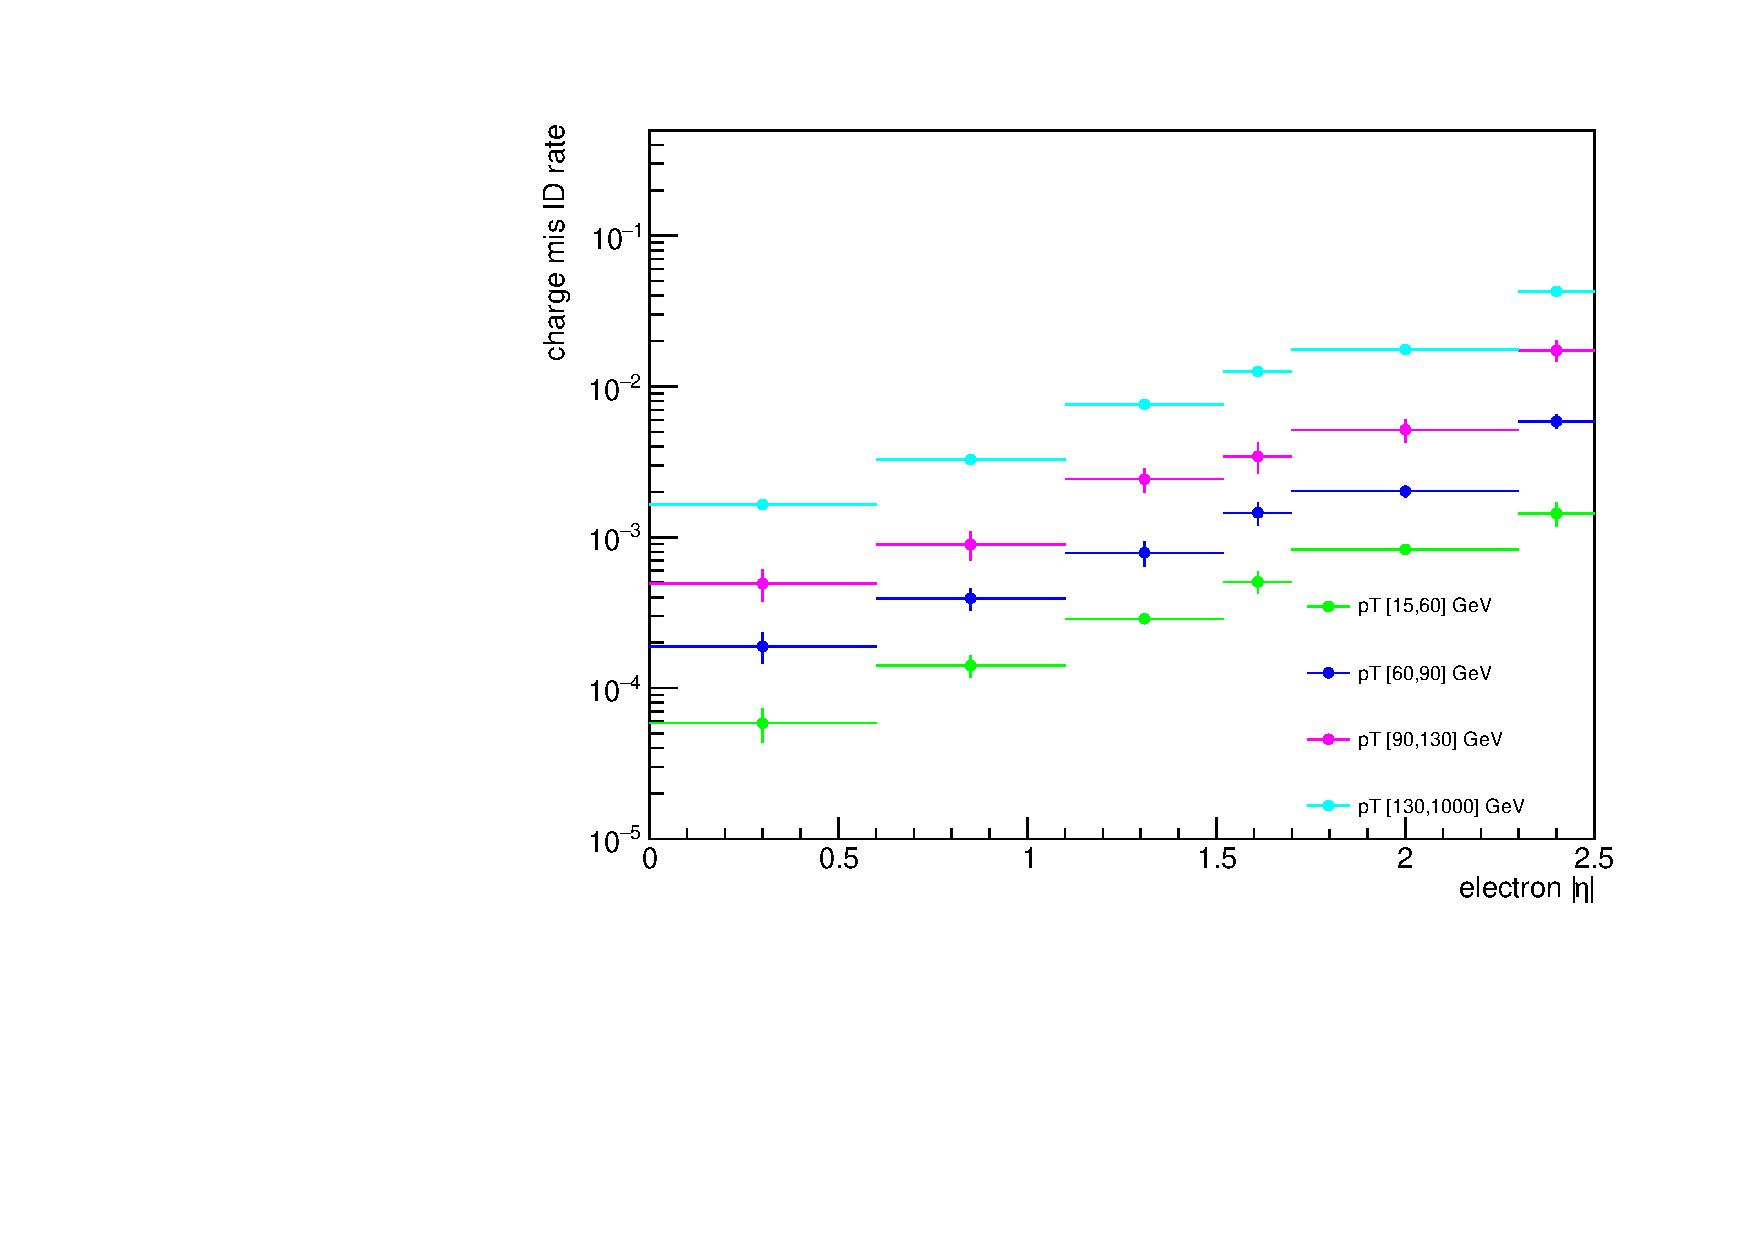
\includegraphics[width=0.5\linewidth]{fig/ana_qmisID_SR_etabins2D.pdf}}
\subfloat[\acs{CR} \ttW]{
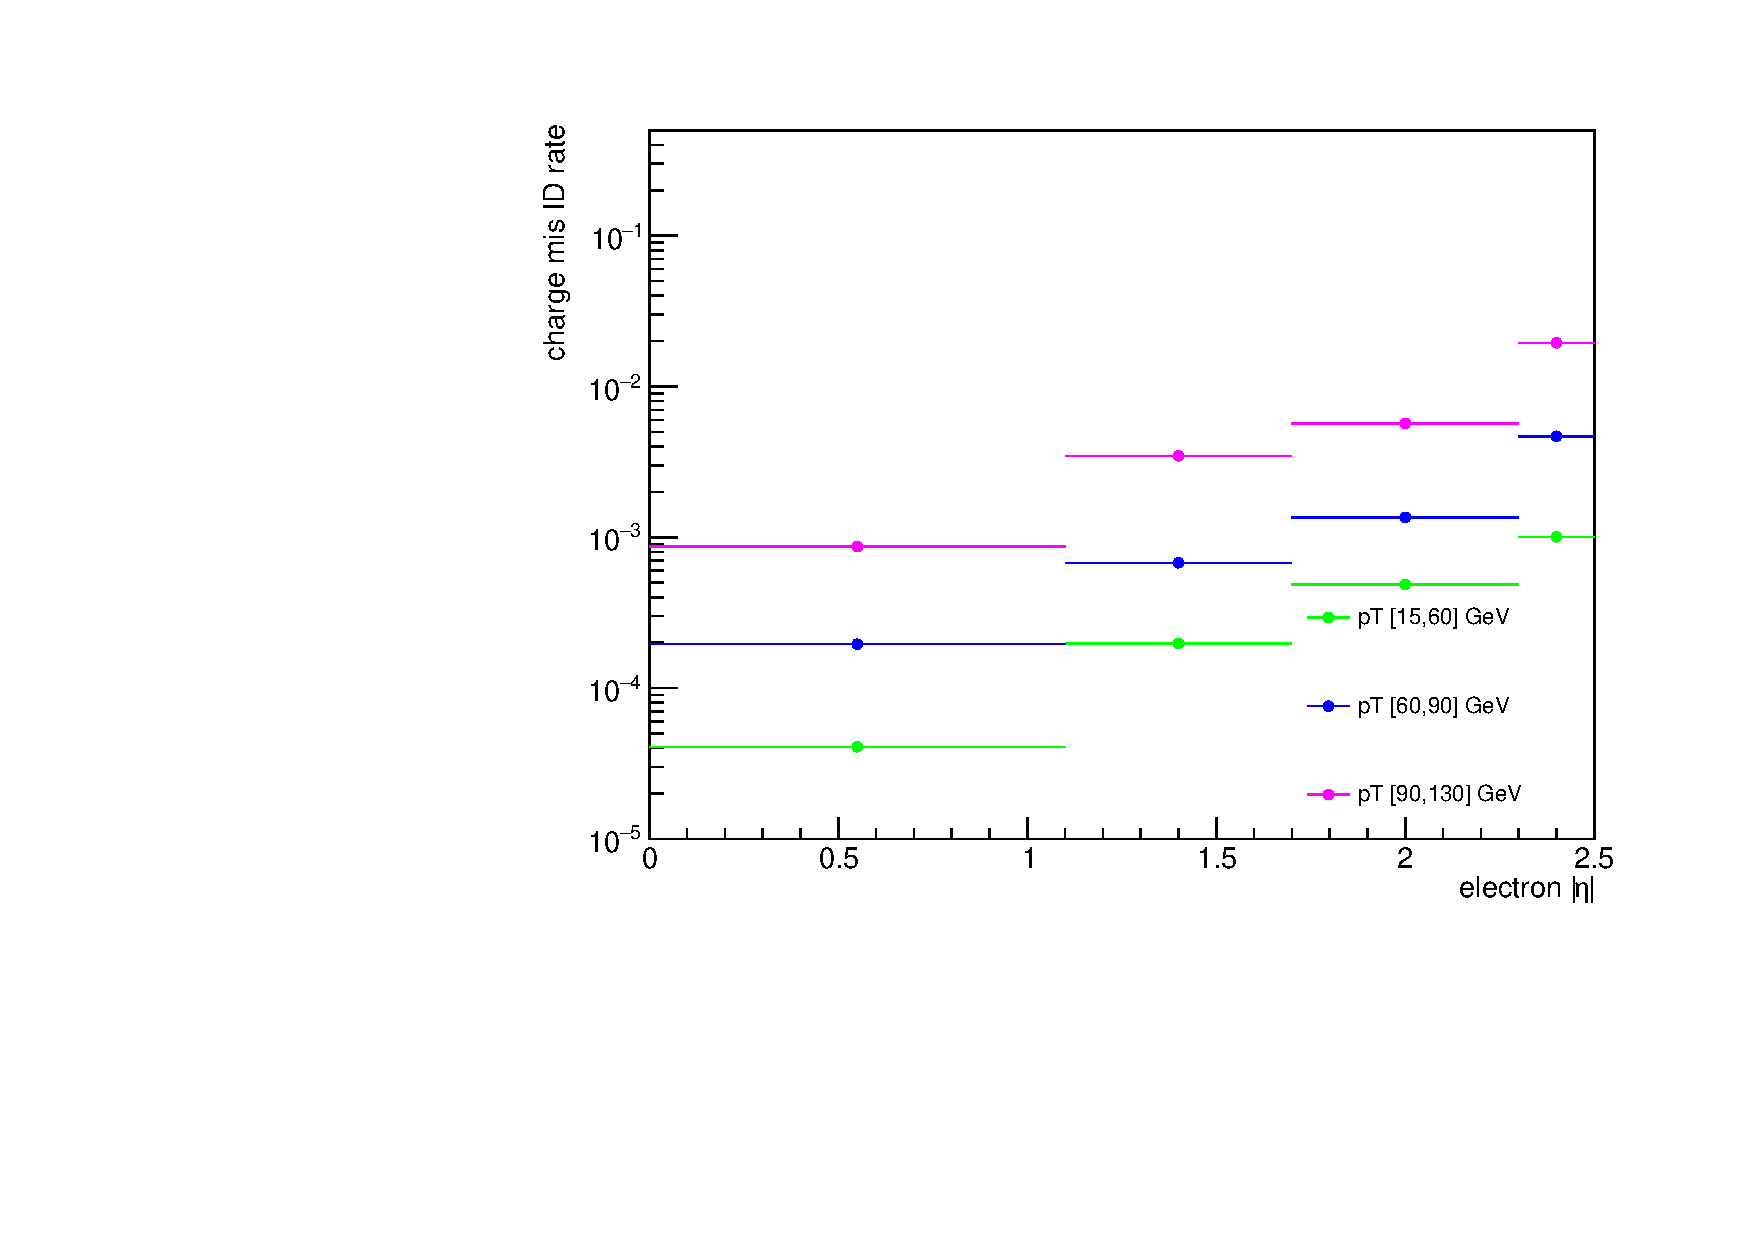
\includegraphics[width=0.5\linewidth]{fig/ana_qmisID_ttW_etabins2D.pdf}}
\caption{\label{fig:ana:qmisid}Charge flip rate calculated for \acs{SR} and \acs{CR} \ttW in bins of $|\eta|$ and \pT.}
\end{figure}

The \acs{QmisID} rates obtained after applying $w$ contain a dependency on jet multiplicity and are underestimated at higher $N_\text{jets}$. This dependency affect the \acs{SR} which require events with $\geq 6$ jets, and is corrected by applying a correction factor $\text{SF}_{i,n} = \epsilon_{i,n}/\epsilon_{i,N}$ where $N$ is the inclusive bin containing all $N_\text{jets}$ and $\epsilon_{i,n}$ is the \acs{QmisID} rate obtained from \autoref{eq:qmisid_llh} in the $(i,n)^\text{th}$ 2D bin in $(\pT, N_\text{jets})$. Jet multiplicity and consequently the obtained \acs{SF}s are assumed to be independent of $|\eta|$.




\subsection{\ttW background data-driven estimation}
\label{sec:ttW_BG}
%- \ttW represents a major source of irreducible background contamination in SM and BSM analyses with \tttt final states.\\
Previously, \ttW background in \tttt final state analysis was handled by assigning large ad-hoc systematic uncertainties to \ttW events with 7 or more jets \citep{tttt_evidence}. A semi-data-driven method \citep{ana:r_par_susy_2021} was shown to be effective in the SM \tttt observation analysis \citep{tttt_obs} by improving \ttW modeling, especially in the showering step and switching \ttW systematic uncertainties from predominantly modeling to statistical.

The data-driven method applies correction factors obtained from a fitted function parameterized in $N_\mathrm{jets}$ to \ttW \acs{MC} kinematic distibutions. The \acs{QCD} scaling patterns \citep{bg:qcd_scaling} can be represented by ratio of successive exclusive jet cross-sections
\begin{equation}
\label{eq:qcd_scaling}
R_{(n+1)/n} = \frac{\sigma_{n+1}}{\sigma_n} = e^{-b} + \frac{\bar{n}}{n+1} = a_0 + \frac{a_1}{1+(j-4)},
\end{equation}
where $a_{0(1)}$ and $b$ are constants, $n$ is the number of jets in addition to the hard process, $j$ is the inclusive number of jets, and $\bar{n}$ is the expectation value for the Poisson distribution of exclusive jet cross-section at jet multiplicity $n$. The \ttW \acs{ME} for \acs{SS2L} events gives 4 jets in the hard process, so $n$ is defined starting from the $5^\text{th}$ jets and the inclusive number of jets $j=n+4$.
%, described as $P_n=\sigma_n/\sigma_\mathrm{tot}$.
%Same-sign dilepton \ttW events dominate the \ttW background and produce $4$ jets in the \acs{ME} at tree level for the hard process
The two terms in \autoref{eq:qcd_scaling} correspond to staircase and Poisson scaling in cross section between successive jet multiplicities and are sensitive to high and low jet multiplicity events respectively \citep{bg:qcd_scaling}.
%For $n+1$ and $n$ jets, staircase scaling is defined as a constant ratio of $e^{-b}$ and is sensitive to events with high $N_\text{jets}$, while Poisson scaling is defined as the ratio between Poisson probabilities and is sensitive to events with low $N_\text{jets}$.
The scaling pattern can then be reparameterized in $a_0$ and $a_1$ to obtain the \ttW yield at $j'\equiv j+1$ jets
\begin{equation}
\mathrm{Yield}_{\ttW(j')} = \mathrm{Yield}_{\ttW(N_\mathrm{jets}=4)} \times 
\mathlarger{\prod}_{j=4}^{j'-1} \left( a_0 + \frac{a_1}{1+(j-4)} \right)
\end{equation}
with $j\geq 4$. The \ttW yield in the 4-jet bin can be represented by a \acs{NF} applied to \ttW \acs{MC} simulation 
\begin{equation}
\mathrm{Yield}_{\ttW(N_\mathrm{jets}=4)}=\mathrm{NF}_{\ttW(N_\mathrm{jets}=4)} \times \mathrm{MC}_{\ttW(N_\mathrm{jets}=4)}.
\end{equation}
To account for the asymmetry in \ttWplus and \ttWminus cross-sections, $\mathrm{NF}_{\ttW(N_\mathrm{jets}=4)}$ is further split into $\mathrm{NF}_{\ttWpm(N_\mathrm{jets}=4)}$ assuming the scaling is the same for both processes. Both \acs{NF}s are left free-floating to constrain \ttW yields in the 4-jet bin within \CRonebp and \CRonebm. The final $N_\mathrm{jets}$-parameterized function can then be represented by $\mathrm{NF}_{\ttW(j')}$ as
\begin{equation}
\label{eq:ttWdd}
\mathrm{NF}_{\ttW(j')} = \left(\mathrm{NF}_{\ttWplus(N_\mathrm{jets}=4)} + \mathrm{NF}_{\ttWminus(N_\mathrm{jets}=4)}\right) \times \mathlarger{\prod}_{j=4}^{j'-1} \left( a_0 + \frac{a_1}{1+(j-4)} \right).
\end{equation}
The normalization is calculated and applied separately for each sub-sample of \ttWplus and \ttWminus in a $N_\mathrm{jets}$ bin for $4\leq N_\mathrm{jets}<10$. Due to small contributions in the \acs{CR}s, events with $N_\mathrm{jets}<4$ and $N_\mathrm{jets}\geq 10$ are not normalized with this scheme. Instead, $N_\mathrm{jets}<4$ events are fitted by propagating normalization in the 4-jet bin without additional shape correction. The correction factor for \ttW events with $N_\mathrm{jets}\geq 10$ is obtained by summing up the overflow from $N_\mathrm{jets}=10$ to $N_\mathrm{jets}=12$, described as $\sum_{j'=10}^{12} \prod_{j=4}^{j'-1}\left(a_0+\frac{a_1}{1+(j-4)}\right)$. Events with $N_\mathrm{jets}\geq 13$ are negligible and are not included in the sum.

The four regions, \CRttWpm and \CRonebpm, are constructed to fit $\mathrm{NF}_{\ttWpm(N_\mathrm{jets}=4))}$ and the scaling parameters $a_{0(1)}$, as well as validating the parameterization. Assuming the $N_\mathrm{jets}$ distribution of \ttW is similar across bins of $N_{b\text{-jets}}$, a fitted $N_\mathrm{jets}$ distribution in \CRonebpm can be used to describe the \ttW parameterization at higher $N_\mathrm{jets}$.
%Validating the \ttW parameterization makes use of the unique charge asymmetry in \ttW production not present in other background or signal processes. The number of events with all negatively charged leptons is subtracted from that of events with all positively charged leptons, which cancels out charge symmetric events and leaves the \ttW background. Validation is done via a statistical-only (stat-only) fit to the \ttW MC prediction in \CRonebpm.
%\subsection{\ttZ background validation}



\end{document}